\documentclass{beamer}
\usetheme{Boadilla}

\usepackage{tikz}
\usepackage{siunitx}
\usepackage{graphicx}

\graphicspath{{img/}}

\title[Physics Problem Solving]{Physics Problem Solving}
\author{Dara Daneshvar \and Eason Shao \and Lev Shabalin}
\institute[]{Physics Problem Solving Society\\St Paul's School}
\date{09.09.2024}

\AtBeginSection[]
{
    \frame{
        \frametitle{Table of Contents}
        \tableofcontents[currentsection]
    }
}

\begin{document}

\frame{\titlepage}

\frame{
    \frametitle{Table of Contents}
    \tableofcontents
}

\section{Welcome!}

\frame{
    \frametitle{Who we are}
    \begin{itemize}
        \item Dara Daneshvar, U8, \url{DaneshD@StPaulsSchool.org.uk}
              \pause
        \item Lev Shabalin, U8, \url{ShabalL@StPaulsSchool.org.uk}
              \pause
        \item Eason Shao, U8, \url{ShaoY@StPaulsSchool.org.uk}
    \end{itemize}
}

\frame{
    \frametitle{What to expect}
    \begin{itemize}
        \item Past Papers for BPhO Competitions
              \pause
        \item Topic-Focused Problem Solving Sessions

              Past examples include:
              \pause
              \begin{itemize}
                  \item Mechanics
                        \pause
                  \item Thermal Physics
                        \pause
                  \item Circuit Analysis
              \end{itemize}
              \pause
        \item Talks by Students

              Past examples include:
              \pause
              \begin{itemize}
                  \item Special Relativity
                        \pause
                  \item Brachistochrone Problem
                        \pause
                  \item Calculus of Variations
              \end{itemize}
    \end{itemize}
}

\frame{
    \frametitle{Our aim}
    \begin{itemize}
        \item Prepare for upcoming BPhO Competitions \url{https://www.bpho.org.uk}
              \pause
        \item Improve problem-solving skills
              \pause
        \item Deepen understanding in physics
    \end{itemize}
}

\section{Overview of BPhO 24-25}

\frame{
    \frametitle{U8 Olympiads}
    \begin{table}
        \begin{tabular}{|p{55pt}|c|c|c|c|c|}
            \hline
            Competition       & Date       & Length      & Format   & U8   & L8   \\
            \hline\hline
            Physics Challenge & Sept - Dec & 1h          & SAQ      & Yes  & Opt. \\
            \hline
            BPhO R1           & 8 Nov      & 1h, 1h40min & SAQ, LAQ & Yes  & PhC  \\
            \hline
            BPhO R2           & 6 Feb      & 3h          & MCQ, LAQ & Inv. & Inv. \\
            \hline
        \end{tabular}
        \caption{BPhO U8 Olympiads}
    \end{table}

    Physics Challenge begins with estimation questions, and has 3 Long Answer Questions.
    \pause

    Note that BPhO R1 has two sections.
    \begin{itemize}
        \item Section 1, 1h, Time-pressured, Short Answer Questions
              \pause
        \item Section 2, 1h40min, Not-as-time-pressured, Long Answer Questions
    \end{itemize}
}

\frame{
    \frametitle{L8 Challenges}
    \begin{table}
        \begin{tabular}{|p{90pt}|c|c|c|c|c|}
            \hline
            Competition                     & Date      & Length    & Format     \\
            \hline\hline
            Senior Physics Challenge Online & 20-24 Jan & 2 * 30min & Online MCQ \\
            \hline
            Senior Physics Challenge        & 7 Mar     & 1h        & MCQ, SAQ   \\
            \hline
        \end{tabular}
        \caption{BPhO L8 Challenges}
    \end{table}

    \url{https://www.bpho.org.uk/Competitions/} for full schedule.
}

\section{Physics Challenge Past Paper}

\frame{
    \frametitle{Qu. 1 Estimations}
    \begin{block}{Qu. 1 (a) [2]}
        What is the equivalent mass of a joule?
    \end{block}

    \pause

    \begin{fact}[Mass-Energy Equivalence Equation]
        \begin{displaymath}
            E = mc^2.
        \end{displaymath}
    \end{fact}
}

\frame{
    \begin{fact}[Mass-Energy Equivalence Equation]
        For stationary particles,
        \begin{displaymath}
            E = mc^2
        \end{displaymath}
        where \(E\) is its energy and \(m\) is its mass.
    \end{fact}

    \pause

    \begin{fact}[Energy-Momentum Relation Equation]
        \begin{displaymath}
            E^2 = (pc)^2 + (m_0 c^2)^2
        \end{displaymath}
        where \(E\) is the total energy of a particle, \(p\) is its momentum, \(m_0\) is its stationary mass and \(c\) is the speed of light.
    \end{fact}
}

\frame{
    \begin{block}{Qu. 1 (c) [4]}
        An inventor designs a novel type of battery reputed to have an emf of \(2 \si{\volt}\) and an internal resistance of \(1 \si{\micro\ohm}\). He claims that this device could deliver \(1 \si{\mega\watt}\) to an appropriate load.

        Comment on the feasibility of this and any safety considerations in the employment of such a power source.
    \end{block}

    \pause

    Draw a circuit diagram!

    \pause

    \begin{fact}
        Maximum power is dissipated to the external load when it has equal resistance with the internal resistance of the power source.
    \end{fact}
}

\frame{
    \begin{fact}
        Maximum power is transferred to the external load when it has equal resistance with the internal resistance of the power source.
    \end{fact}

    \begin{solution}
        When the maximum power is obtained, the load has resistance of \(R = r = 1\si{\micro\ohm}\) as well.
        \pause

        Therefore, by Ohm's law, the current \(I = \frac{\mathcal{E}}{R + r} = \frac{2\si{\volt}}{2\si{\micro\ohm}} = 1\si{\mega\ampere}\).
        \pause

        Therefore, the power \(P = I^2 R = (1 \si{\mega\ampere})^2 \cdot 1\si{\micro\ohm} = 1 \si{\mega\watt}\) as claimed.
    \end{solution}
}

\frame{
    \frametitle{Qu. 2 Stopping Distances}
    \begin{block}{Qu. 2(a). [2 + 2]}
        \begin{itemize}
            \item What is the kinetic energy of a car of mass \(1000 \si{\kilogram}\) travelling at \(30 \si{\metre\per\second}\)?
            \item A car travelling at approximately \(30 \si{\metre\per\second}\) in the country is required by law to halve its speed on entering a built-up area. What fraction of its kinetic energy is lost in doing this?
        \end{itemize}
    \end{block}
}

\frame{
    \begin{figure}
        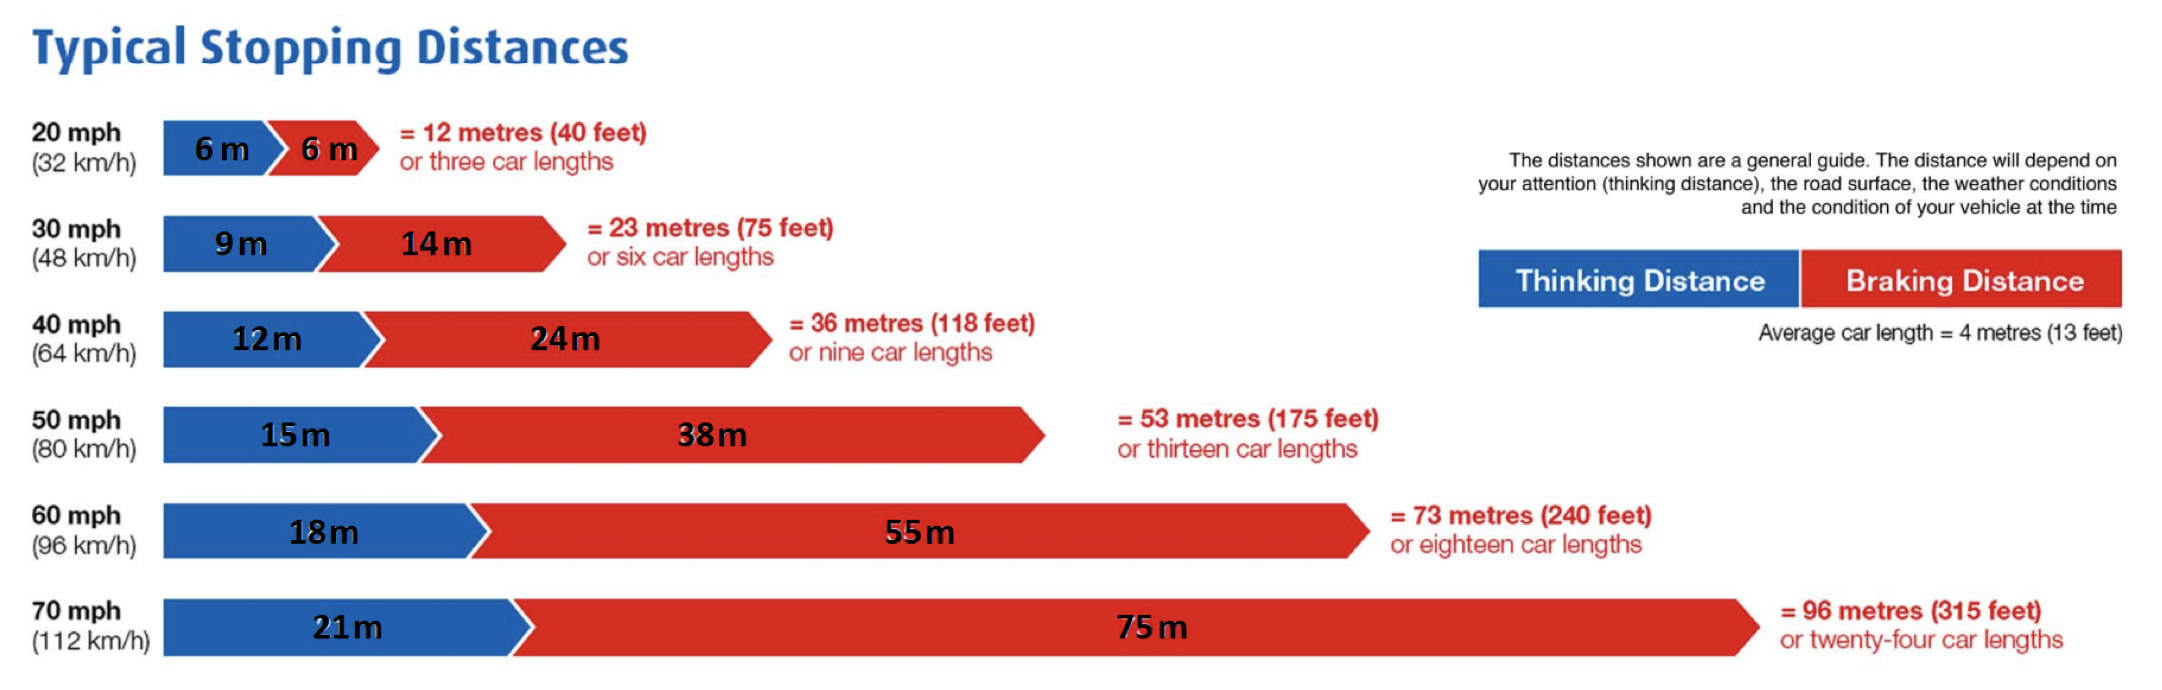
\includegraphics[width=0.75\linewidth]{stoppingDistances.png}
        % \caption{A table of stopping distances taken from the Highway Code.}
    \end{figure}

    \begin{block}{Qu. 2(b). [1 + 1]}
        \begin{itemize}
            \item By inspection of the values given in the figure, suggest a relationship between the thinking distance, \(T\), and the speed, \(v\).
            \item The Thinking Distance in the table derives from empirical information about the behaviour of drivers. If you were to propose a theoretical explanation of this phenomenon, what assumption would be needed to explain your suggested relationship?
        \end{itemize}
    \end{block}
}

\frame{
    \begin{block}{Qu. 2(c) i. [3]}
        Clearly, the speed and stopping distance have a different relationship. A student who has seen part (a) of this question suggests that the braking distance, \(B\), is proportional to the square of the speed, \(v^2\).

        Using the data, devise a test to check this hypothesis and comment on the results of your test.
    \end{block}
    \pause

    \begin{solution}
        \begin{enumerate}
            \item Draw a table, with \(B\) as a column, \(v^2\) as a column, and \(B / v^2\) as the final column. Compare the final column values.
                  \pause
            \item Draw a graph, with \(B\) on the \(y\)-axis, \(v^2\) on the \(x\)-axis, and verify they are all lying close to line of best fit.
        \end{enumerate}
    \end{solution}
}

\frame{
    \begin{block}{Qu. 2(c) ii. [1]}
        Again, the observed relationship is only an empirical finding. If you were to devise a theoretical explanation of the \(B \propto v^2\) relationship, what assumption would you need to make about the braking behaviour of a car?
    \end{block}
}

\frame{
    \begin{fact}[\(suvat\) equations]
        For motion with uniform acceleration \(a\), initial speed \(v\), final speed \(u\), elapsed time \(t\) and displacement \(s\), we must have:
        \begin{displaymath}
            \begin{cases}
                a = \frac{v - u}{t}      \\
                s = ut + \frac{1}{2}at^2 \\
                s = vt - \frac{1}{2}at^2 \\
                s = \frac{1}{2}(u + v)t  \\
                2as = v^2 - u^2          \\
            \end{cases}
        \end{displaymath}
    \end{fact}
}

\frame{
    \begin{block}{Qu. 2(c) iii. [3]}
        Calculate the deceleration of a car when it brakes from a speed of \(80 \si{\kilo\metre\per\hour}\).
    \end{block}
    \pause

    Units!
    \begin{fact}
        \(1 \si{\metre\per\second} = 3.6 \si{\kilo\metre\per\hour}.\)
    \end{fact}
}

\frame{
    \begin{block}{Qu. 2(c) iv. [2]}
        Hence determine the (minimum) coefficient of (static) friction, \(\mu\), for contact between car tyres and the road. (\(\mu\) is the ratio of the maximum braking force before skidding sets in, to the weight of the car).
    \end{block}
    \pause

    \begin{solution}
        \begin{displaymath}
            \mu = \frac{ma}{mg} = \frac{a}{g} = \ldots
        \end{displaymath}
    \end{solution}

    Try doing cancellation before actually plugging in the values (and don't be afraid of setting unknowns).
}

\frame{
    \begin{block}{Qu. 2(c) v. [2]}
        It is often stated (incorrectly) that the value of \(\mu\) cannot exceed unity. But, if tyres had this excellent level of grip, what would be the minimum stopping distance from \(96 \si{\kilo\metre\per\hour}\)?
    \end{block}
}

\end{document}